% LinkedIn carousel: sparse slide version of
% Main_TwoPager_MidcurveNN_GeometryResearch.tex
%
% Square 1:1 (1080x1080 equivalent) -- LinkedIn renders carousel PDFs best at
% 1:1 or 4:5. Upload the PDF directly as a document post.
%
% Build:  texify --engine=xetex -cp Main_Carousel_MidcurveNN_GeometryResearch.tex
%
% NOTE ON PAGE SIZE: beamer has no aspectratio=11 option (tried, 100 errors).
% Beamer loads geometry itself, so re-invoking \geometry afterwards is what
% actually resizes the page. Do not replace this with a class option.

% 't' top-aligns frame content. Without it beamer vertically centres each
% frame, which on a square page leaves a large gap between the title rule and
% the first line.
\documentclass[11pt,t]{beamer}

\usetheme{default}
\usecolortheme{default}
\setbeamertemplate{navigation symbols}{}
\setbeamertemplate{footline}{}
\geometry{papersize={128mm,128mm}}
\setbeamersize{text margin left=9mm,text margin right=9mm}

\usepackage[T1]{fontenc}
\usepackage{graphicx}
\usepackage{tikz}
\usepackage{microtype}

\graphicspath{{images/}}

\definecolor{ink}{HTML}{16233A}
\definecolor{accent}{HTML}{1F6F8B}
\definecolor{warn}{HTML}{B4432E}
\definecolor{muted}{HTML}{6C7A89}
\definecolor{paper}{HTML}{FBFAF7}

\setbeamercolor{background canvas}{bg=paper}
\setbeamercolor{normal text}{fg=ink}
\setbeamercolor{frametitle}{fg=ink}
\setbeamerfont{frametitle}{series=\bfseries,size=\Large}
\setbeamertemplate{frametitle}{%
  \vspace{6mm}\usebeamerfont{frametitle}\insertframetitle\par
  \vspace{1mm}{\color{accent}\rule{18mm}{1.2pt}}\par\vspace{2mm}}

\newcommand{\slidenum}[1]{%
  \begin{tikzpicture}[remember picture,overlay]
    \node[anchor=south east,inner sep=5mm,text=muted,font=\scriptsize]
      at (current page.south east) {#1\,/\,12};
  \end{tikzpicture}}

\newcommand{\kicker}[1]{{\color{accent}\bfseries\footnotesize\MakeUppercase{#1}}\par\vspace{1.5mm}}

\begin{document}

% ---------------------------------------------------------------- 1: title
\begin{frame}[plain]
\vspace{10mm}
{\color{accent}\bfseries\footnotesize RESEARCH TOPIC \textbullet\ MS / PhD}\par
\vspace{5mm}
{\Huge\bfseries Learning the\\[1mm] Medial Axis\par}
\vspace{5mm}
{\color{accent}\rule{28mm}{1.4pt}}\par
\vspace{5mm}
{\large Why a neural network can find\\ the middle of a shape ---\\ but not how it connects.\par}
\vfill
{\footnotesize\color{muted} Yogesh H. Kulkarni \quad$\cdot$\quad github.com/yogeshhk/MidcurveNN\par}
\vspace{4mm}
\slidenum{1}
\end{frame}

% ---------------------------------------------------------------- 2: problem
\begin{frame}{The problem}
\kicker{one sentence}
{\large Given a closed 2D shape, find the polyline running down its middle.\par}
\vspace{6mm}
\begin{center}
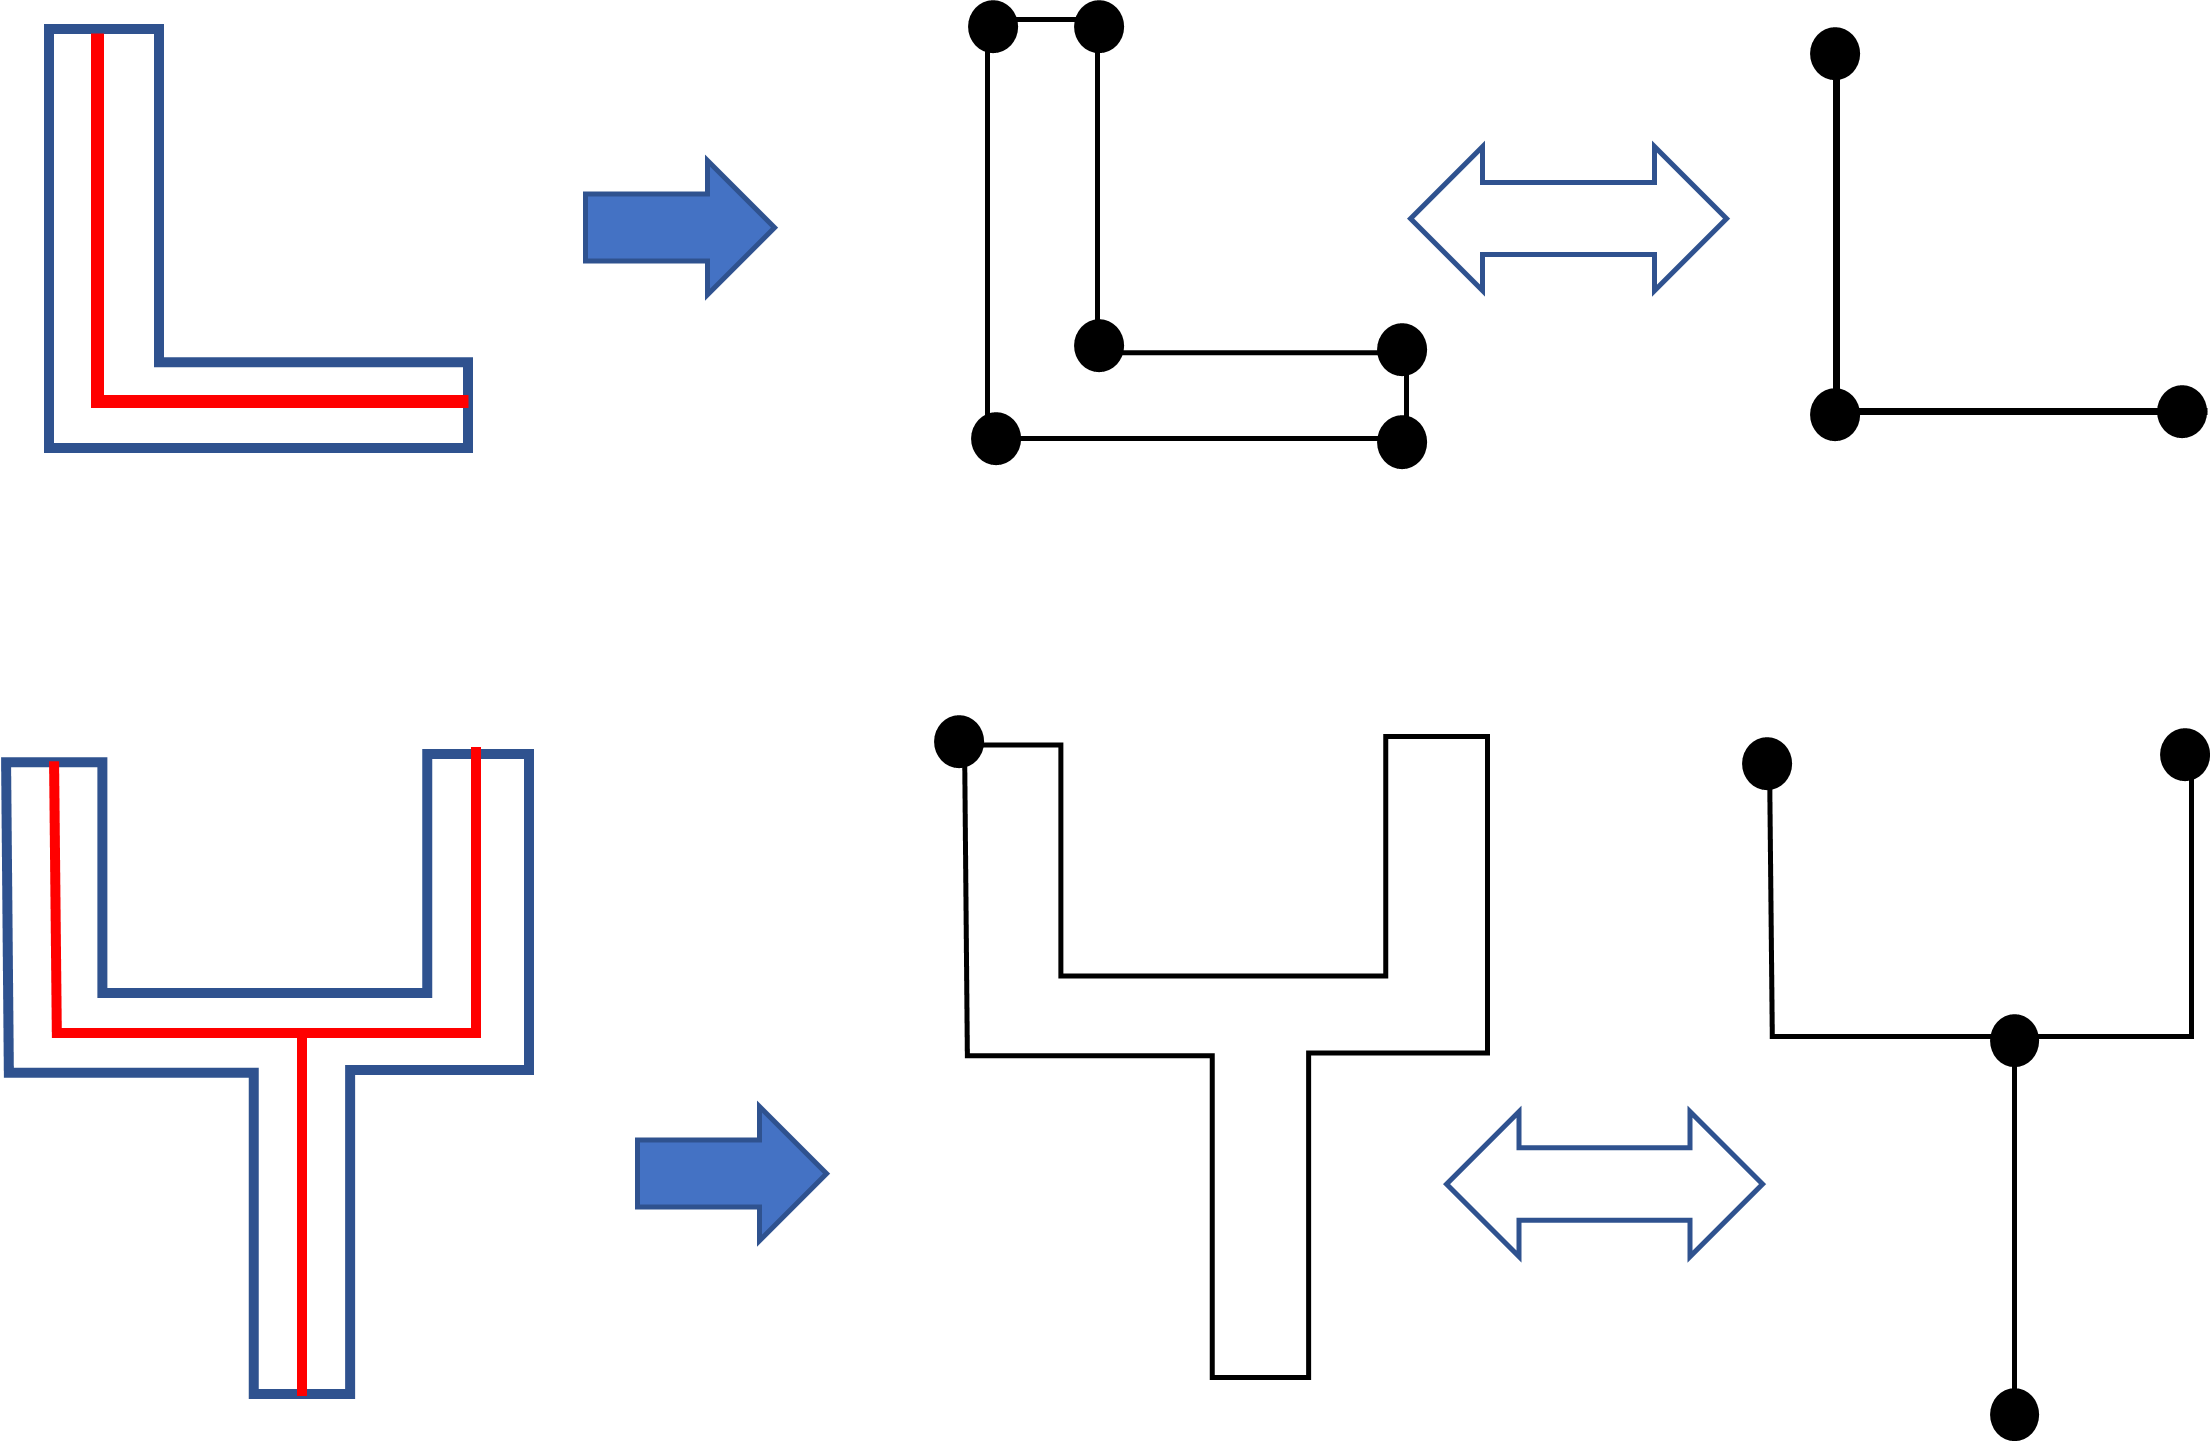
\includegraphics[width=0.86\linewidth,keepaspectratio]{midcurve_as_graph}
\end{center}
\vfill
{\footnotesize\color{muted} Sounds narrow. It is not.\par}
\slidenum{2}
\end{frame}

% ---------------------------------------------------------------- 3: why
\begin{frame}{Why it matters}
\vspace{2mm}
{\large Every thin part headed for structural simulation gets\\ reduced to a simpler idealization first.\par}
\vspace{7mm}
{\large Done well: \textbf{10x cheaper} simulation.\par}
\vspace{3mm}
{\large Done badly: \textbf{\color{warn}silently wrong} physics.\par}
\vspace{7mm}
{\large In production CAD this is still\\ \textbf{largely done by hand.}\par}
\slidenum{3}
\end{frame}

% ---------------------------------------------------------------- 4: attempt 1
\begin{frame}{Attempt 1 --- pixels}
\kicker{rasterize, learn image to image}
\vspace{2mm}
{\large It works. Seven encoder--decoder variants,\\ UNet strongest.\par}
\vspace{8mm}
{\large \textbf{\color{warn}But the output is pixels.}\par}
\vspace{4mm}
{\large Getting a clean polyline back out of a fuzzy\\ raster is a second unsolved problem.\par}
\vspace{4mm}
{\large Exact coordinates, connectivity, branch points ---\\ all discarded at the input.\par}
\slidenum{4}
\end{frame}

% ---------------------------------------------------------------- 5: attempt 2
\begin{frame}{Attempt 2 --- text}
\kicker{serialize to json, fine-tune an llm}
\vspace{2mm}
{\large Best performer so far. Exact coordinates,\\ explicit topology.\par}
\vspace{8mm}
{\large \textbf{\color{warn}But it learns a serialization convention,}\\ \textbf{\color{warn}not a geometric operation.}\par}
\vspace{5mm}
{\large No invariance guarantees under rotation or scale.\par}
\vspace{3mm}
{\large And it takes \textbf{7 billion parameters} for a problem\\ whose intrinsic dimension is tiny.\par}
\slidenum{5}
\end{frame}

% ---------------------------------------------------------------- 6: pattern
\begin{frame}[plain]
\vspace{22mm}
\begin{center}
{\Large Both route a\par}
\vspace{2mm}
{\Huge\bfseries\color{accent} geometric problem\par}
\vspace{2mm}
{\Large through a representation\\ that is not geometric.\par}
\end{center}
\vfill
\slidenum{6}
\end{frame}

% ---------------------------------------------------------------- 7: attempt 3
\begin{frame}{Attempt 3 --- geometry}
\kicker{predict geometry as geometry}
{\large Shape in as a \textbf{graph}. Midcurve out as a \textbf{graph}.\\ Exact coordinates throughout.\par}
\vspace{4mm}
\begin{center}
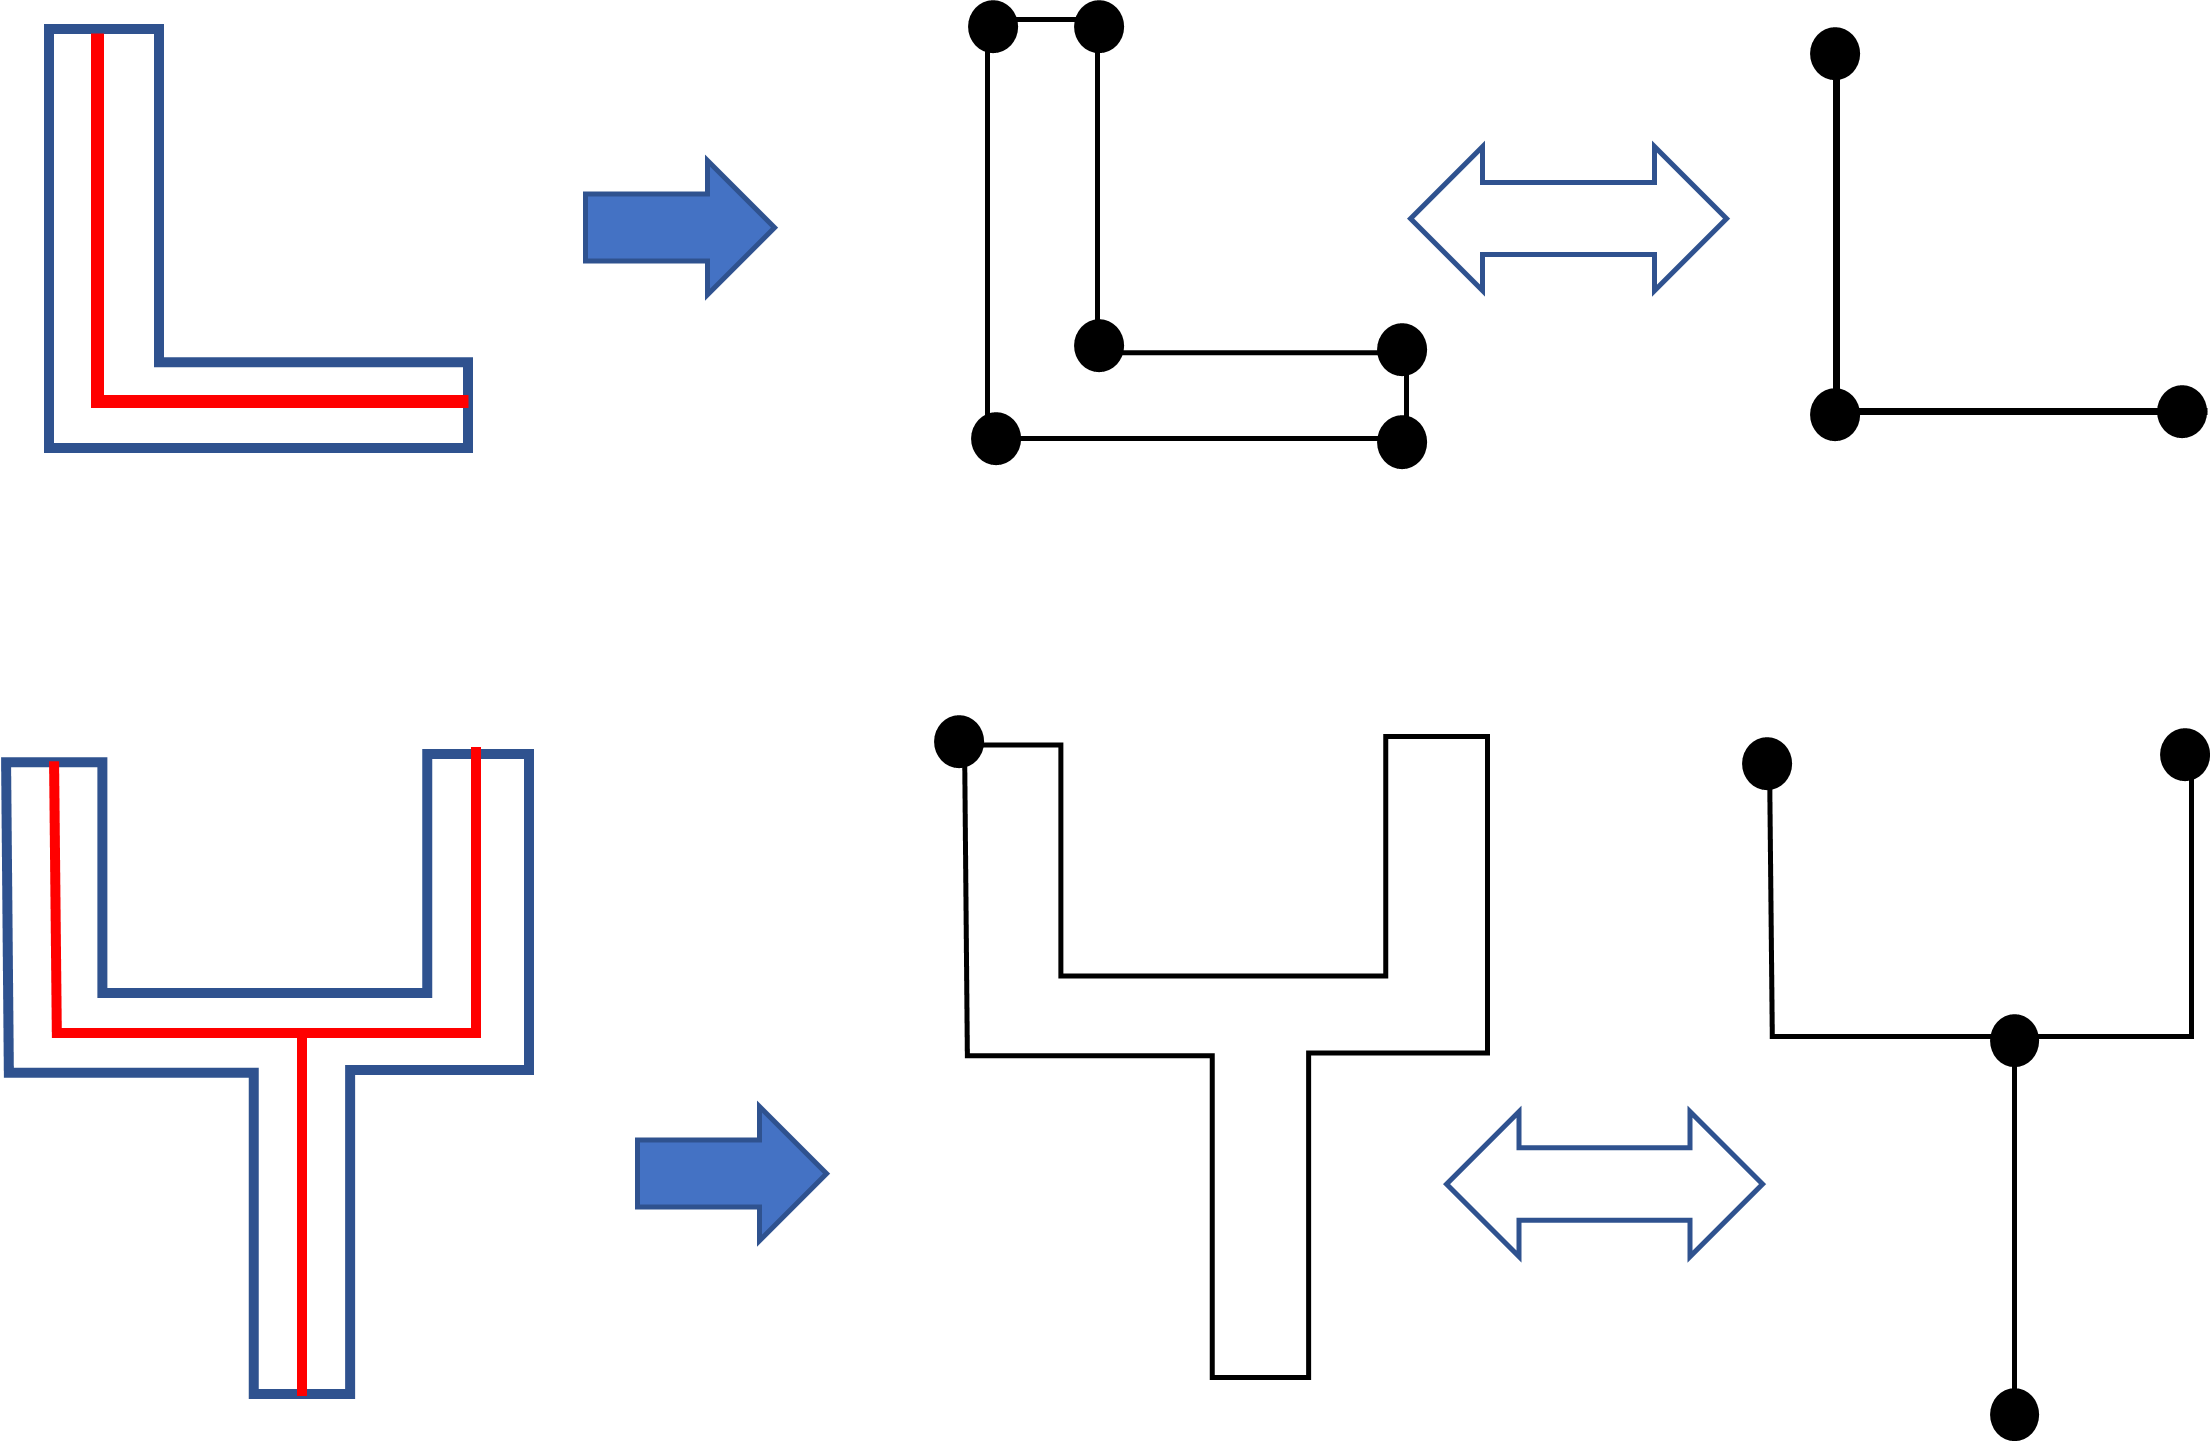
\includegraphics[width=0.78\linewidth,keepaspectratio]{midcurve_as_graph}
\end{center}
\vspace{2mm}
{\large Branching is native. Invariances can be built in.\par}
\slidenum{7}
\end{frame}

% ---------------------------------------------------------------- 8: result
\begin{frame}{What happened}
\begin{center}
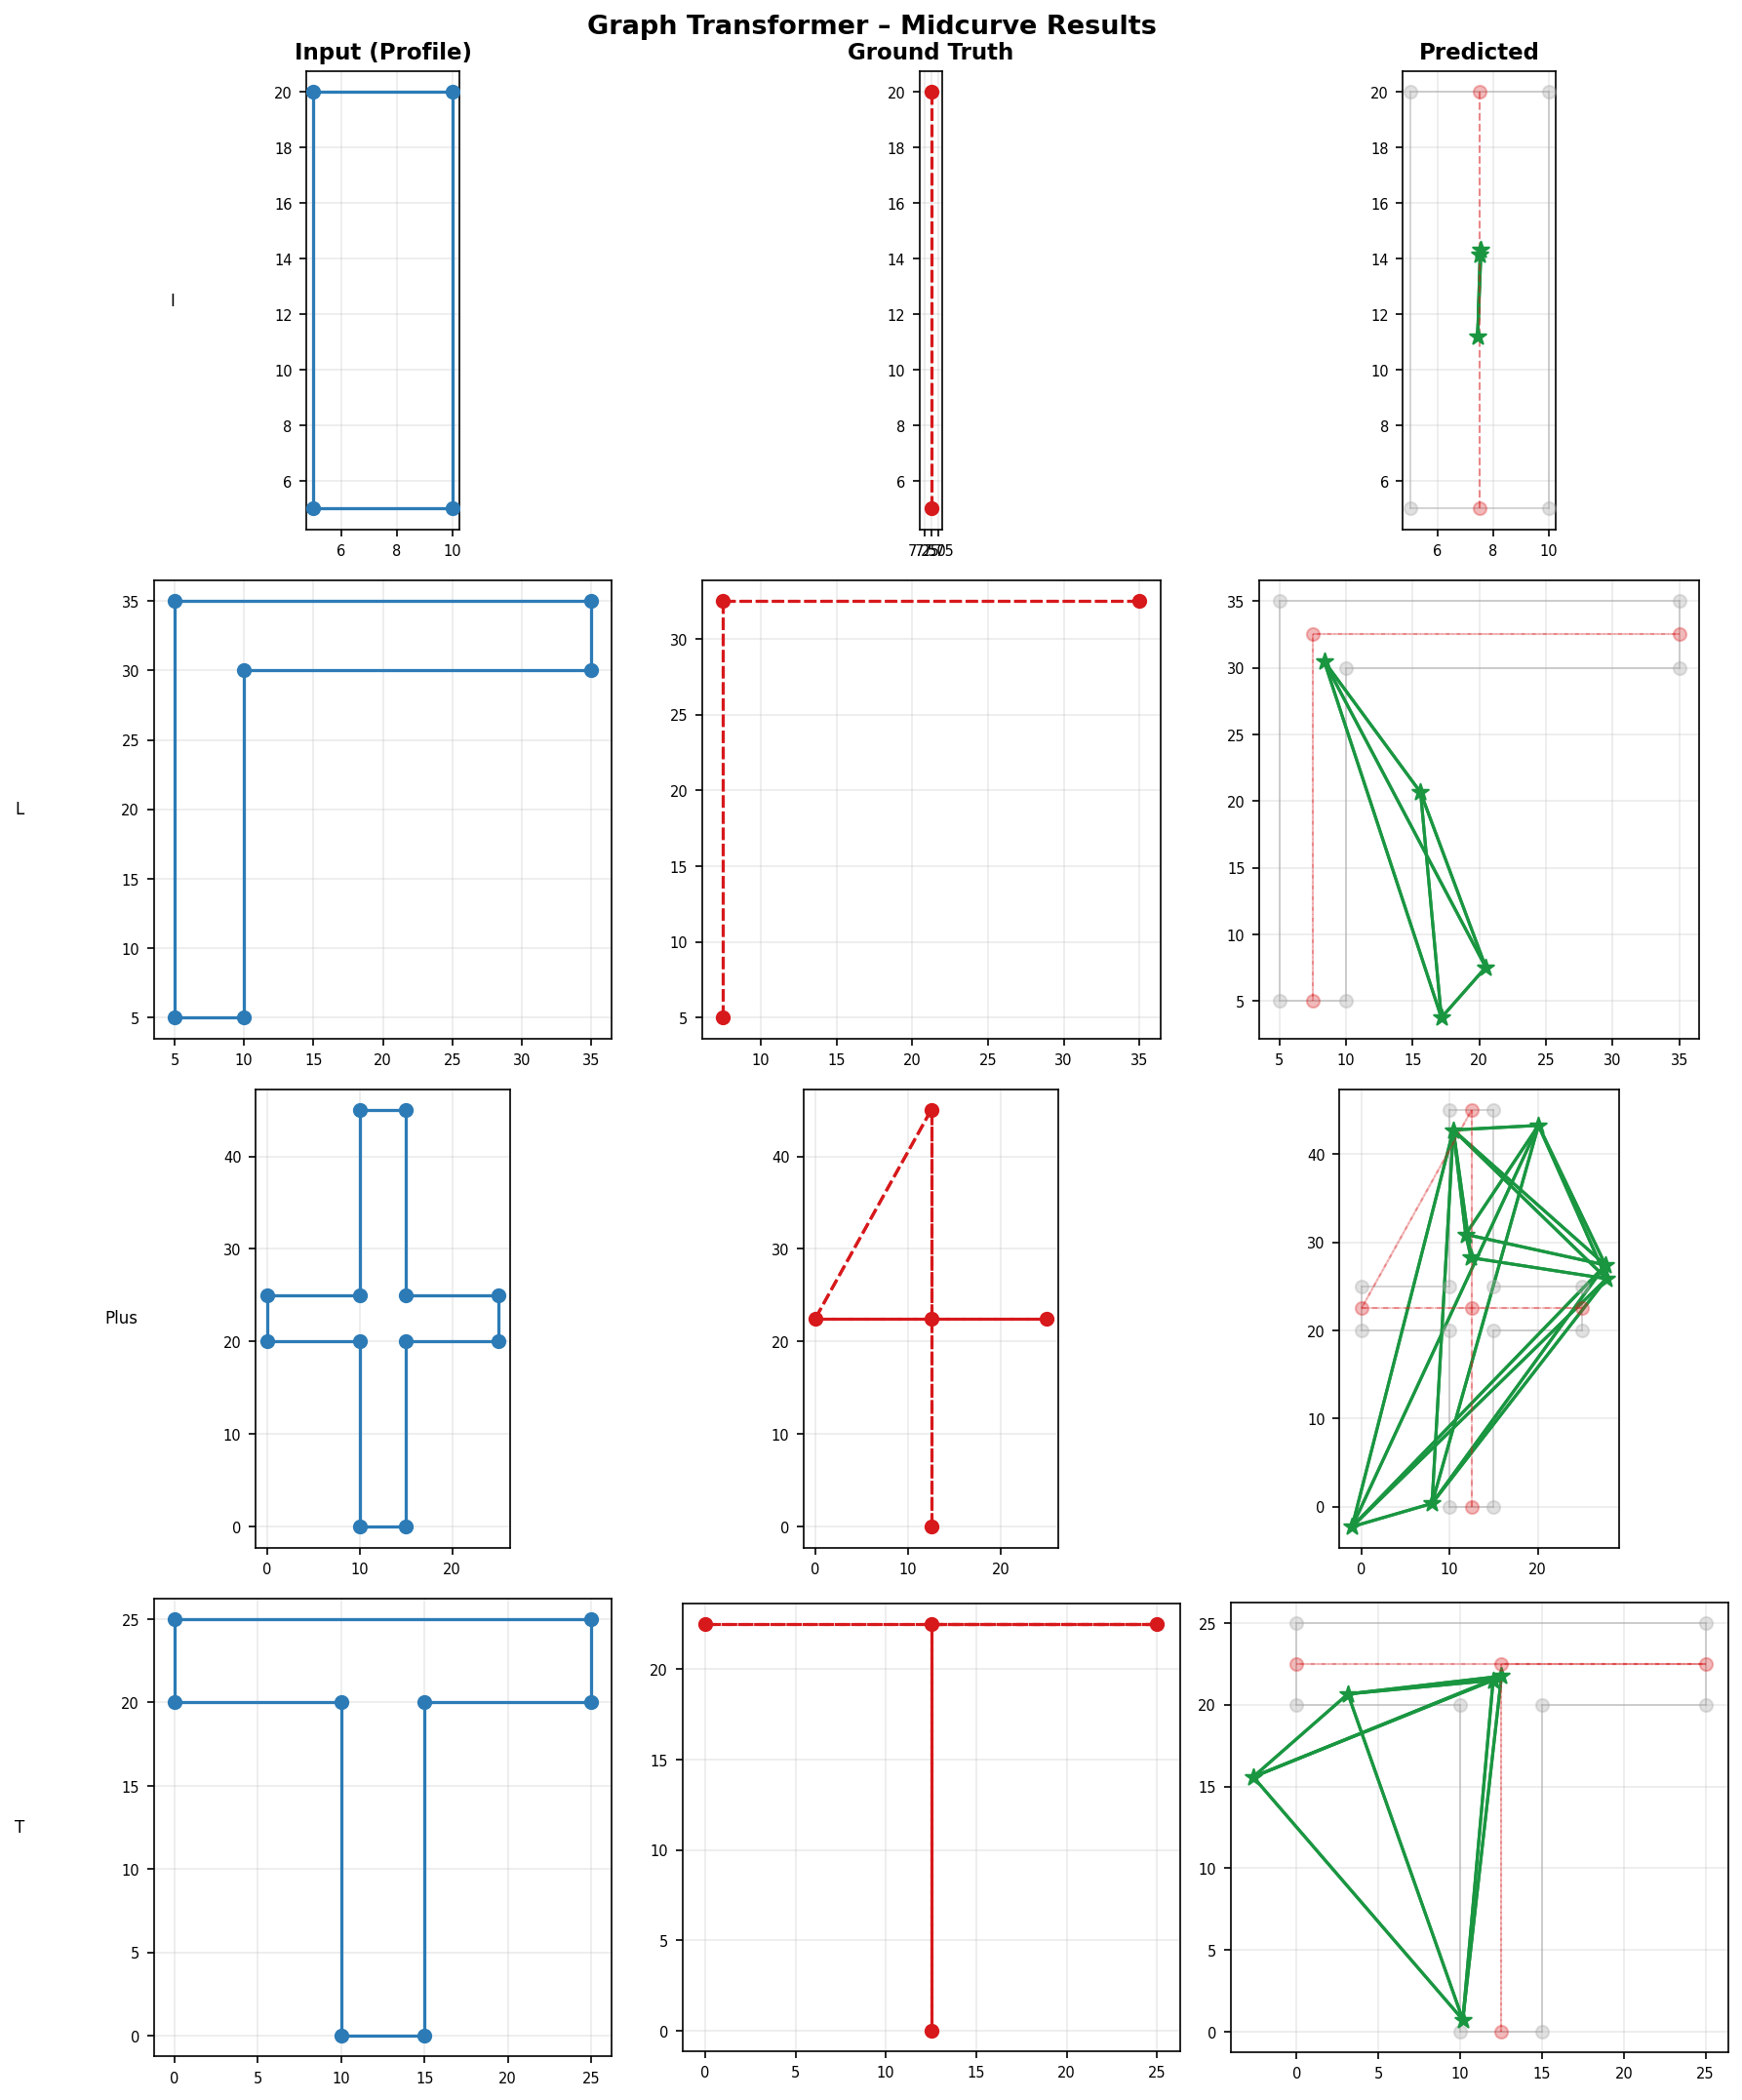
\includegraphics[width=0.52\linewidth,keepaspectratio]{graph_transformer_results_grid}
\end{center}
\vspace{1mm}
{\large It learns \textbf{where} the points go.\par}
\vspace{1.5mm}
{\large It does \textbf{\color{warn}not} learn how they connect.\par}
\vspace{2mm}
{\footnotesize\color{muted} Adjacency cross-entropy $\approx 1.15$ --- indistinguishable from chance.\par}
\slidenum{8}
\end{frame}

% ---------------------------------------------------------------- 9: Q1 Q2
\begin{frame}{Not a tuning problem}
\kicker{open question 1}
{\large \textbf{Output sets of unknown size,}\\ \textbf{with no correspondence.}\par}
\vspace{2mm}
{\footnotesize\color{muted} Nothing tells the loss which predicted node matches which true one. Chamfer distance sidesteps it and gives no gradient for topology.\par}
\vspace{7mm}
\kicker{open question 2}
{\large \textbf{Topology as a real target.}\par}
\vspace{2mm}
{\footnotesize\color{muted} A midcurve is connected, essentially acyclic, and its branch points carry engineering meaning. Independent Bernoulli entries encode none of that.\par}
\slidenum{9}
\end{frame}

% ---------------------------------------------------------------- 10: Q3 Q4
\begin{frame}{Not a tuning problem}
\kicker{open question 3}
{\large \textbf{Long-range geometric reasoning.}\par}
\vspace{2mm}
{\footnotesize\color{muted} A midcurve point is equidistant from two \emph{opposing} walls --- maximally far apart in graph distance. Three rounds of message passing cannot pair them.\par}
\vspace{7mm}
\kicker{open question 4}
{\large \textbf{Generalization from four shapes.}\par}
\vspace{2mm}
{\footnotesize\color{muted} The dataset has four base topologies. Every reported number measures interpolation, not generalization. Honest evaluation needs leave-one-shape-out and synthetic data.\par}
\slidenum{10}
\end{frame}

% ---------------------------------------------------------------- 11: scope
\begin{frame}{Two ways in}
\vspace{3mm}
\kicker{master's --- one year}
{\large Questions \textbf{1} and \textbf{4}.\par}
\vspace{1mm}
{\footnotesize\color{muted} Set-prediction decoder with Hungarian matching; synthetic data generator; the first honest generalization number for this problem.\par}
\vspace{9mm}
\kicker{doctoral --- three to four years}
{\large All four, plus \textbf{midsurfaces}.\par}
\vspace{1mm}
{\footnotesize\color{muted} Closed to open, manifold to non-manifold. A thin solid reduces not to one sheet but to several meeting at non-manifold junctions. Learning maps whose output topology differs structurally from their input.\par}
\slidenum{11}
\end{frame}

% ---------------------------------------------------------------- 12: CTA
\begin{frame}[plain]
\vspace{12mm}
{\color{accent}\bfseries\footnotesize LOOKING FOR STUDENTS}\par
\vspace{4mm}
{\LARGE\bfseries What you get\par}
\vspace{5mm}
{\large Three implemented approaches\\ to benchmark against.\par}
\vspace{3mm}
{\large A working evaluation harness.\par}
\vspace{3mm}
{\large A blunt written record of everything\\ currently broken --- down to file and line.\par}
\vspace{8mm}
{\large\bfseries github.com/yogeshhk/MidcurveNN\par}
\vspace{3mm}
{\footnotesize\color{muted} Two-page topic summary in the repo. Students and co-supervisors welcome.\par}
\slidenum{12}
\end{frame}

\end{document}
